\documentclass[conference]{IEEEtran}
\IEEEoverridecommandlockouts
\usepackage{amsmath,amssymb,amsthm}
\usepackage{graphicx}
\usepackage{booktabs}
\usepackage{xcolor}
\usepackage{pifont}
\usepackage{tikz}
\usetikzlibrary{arrows.meta,positioning,calc}
\usepackage[hidelinks]{hyperref}
\graphicspath{{../figures/}}
\renewcommand{\ttdefault}{cmtt}
% generated by experiments/make_macros.py -- do not edit
\newcommand{\RPairMs}{1{,}403}
\newcommand{\RMulMs}{6.87}
\newcommand{\RSmallMulMs}{1.39}
\newcommand{\RPairRatio}{44}
\newcommand{\RAvailIidHalfOne}{50.3}
\newcommand{\RAvailIidHalfThree}{87.5}
\newcommand{\RAvailBurstHalfThree}{59.2}
\newcommand{\RNmax}{100}
\newcommand{\ROursTotalS}{6.49}
\newcommand{\RBaseTotalS}{388}
\newcommand{\RBaseTuavS}{0.21}
\newcommand{\RBaseTaS}{384}
\newcommand{\RPerUavOursMs}{64.9}
\newcommand{\RPerUavBaseS}{3.84}
\newcommand{\RMeasRatioLo}{56}
\newcommand{\RMeasRatioHi}{67}
\newcommand{\RCountRatioLo}{55}
\newcommand{\RCountRatioHi}{66}
\newcommand{\RSpeedup}{65}
\newcommand{\ROutlierRatio}{107}
\newcommand{\RBaseTuavShare}{0.05}
\newcommand{\RPoisonN}{60}
\newcommand{\RPoisonClean}{2.00}
\newcommand{\RPoisonWorst}{7.00}
\newcommand{\RPoisonIndiv}{4.83}
\newcommand{\RPoisonGoodTwenty}{80}
\newcommand{\RBytesBaseKey}{17.5}
\newcommand{\RBytesOursKey}{9.6}
\newcommand{\RBytesBaseSat}{158.6}
\newcommand{\RBytesRatio}{1{,}823}
\newcommand{\RReqBase}{137}
\newcommand{\RReqOurs}{225}
\newcommand{\RVehN}{500}
\newcommand{\RVehBatchS}{29.6}
\newcommand{\RVehIndS}{39.2}
\newcommand{\RVehDropUs}{15}
\newcommand{\RHoTuavFull}{105.0}
\newcommand{\RHoTuavTicket}{52.3}
\newcommand{\RHoMemFull}{150.8}
\newcommand{\RHoMemTicket}{50.7}
\newcommand{\RHoCross}{557}
\newcommand{\RHoGapFull}{756}
\newcommand{\RHoGapTicket}{103}
\newcommand{\RHoCpuFull}{58.5}
\newcommand{\RHoCpuTicket}{29.1}


\definecolor{deep}{HTML}{0B3954}\definecolor{uavc}{HTML}{087E8B}\definecolor{vehc}{HTML}{6A4C93}
\definecolor{hoc}{HTML}{E07A1F}\definecolor{bad}{HTML}{C81D25}\definecolor{good}{HTML}{2A9D3F}
\newcommand{\yes}{\textcolor{good}{\ding{51}}}
\newcommand{\no}{\textcolor{bad}{\ding{55}}}
\newcommand{\Ppub}{P_{\mathrm{pub}}}
\newcommand{\Tpub}{T_{\mathrm{pub}}}
\newcommand{\PID}{\mathit{PID}}
\newcommand{\RID}{\mathit{RID}}
\newcommand{\GK}{\mathit{GK}}
\newcommand{\VK}{\mathit{VK}}
\newcommand{\pk}{\mathit{pk}}
\newcommand{\sk}{\mathit{sk}}
\newcommand{\ep}{\mathit{ep}}
\newcommand{\cat}{\,\|\,}
\newcommand{\Enc}{\mathsf{Enc}}
\newcommand{\KDF}{\mathsf{KDF}}
\newcommand{\MAC}{\mathsf{MAC}}
\newtheorem{theorem}{Theorem}
\newtheorem{lemma}{Lemma}
\newtheorem{proposition}{Proposition}

\begin{document}

\title{Cutting the Cord: Authority-Independent, Escrow-Free Authentication and Key Management for TUAV-Assisted Infrastructure-Less IoV}

\author{\IEEEauthorblockN{Swaraj Kumar, Hritik Ranjan, Harsh Raj}
\IEEEauthorblockA{Team 6 --- Research in Information Security, October 2026}}

\maketitle

\begin{abstract}
A recent scheme by Tan, Zheng and Vijayakumar (IEEE T-ITS 2023) uses a tethered UAV (TUAV) to replace roadside units destroyed by a disaster, so that an
Internet of Vehicles keeps working ``without infrastructure''. We show that it does not achieve this. Every authentication is relayed over a satellite link
to a cloud Trusted Authority (TA) that computes all pairings. The UAV credential depends only on values the TA holds, so the TA can impersonate any UAV.
The CRT-based group key reveals every member's decrypting key to every other member, so a revoked UAV still obtains the new key. The reported costs omit the
TA's pairings and an $O(n^3)$-byte key broadcast. We confirm these findings in code and, for the escrow attack, with ProVerif. We then propose
\emph{Cutting the Cord}, which moves the trust root offline. The TUAV authenticates UAVs itself with escrow-free, pairing-free certificateless signatures in a
sound batch with a bounded fallback. It delivers the group key per member under fresh ECDH keys, admits vehicles through authenticated UAV relays, and hands
members between TUAVs with single-use tickets. ProVerif verifies authentication, key secrecy, forward secrecy and revocation, and delimits the residual TA power
to Girault level~2. On the same curve and library, the base scheme's TA-inclusive cost is about \RSpeedup$\times$ ours, our scheme needs no satellite traffic, and it
sends \RBytesRatio$\times$ less key traffic.
\end{abstract}

\begin{IEEEkeywords}
Internet of Vehicles, tethered UAV, certificateless signatures, batch verification, group key management, ProVerif.
\end{IEEEkeywords}

% =====================================================================
\section{Introduction}
Roadside units (RSUs) authenticate vehicles in a conventional Internet of Vehicles (IoV). After an earthquake or flood they are among the first things to fail,
exactly when rescue traffic needs secure coordination. Tan \textit{et al.}~\cite{base} propose a \emph{tethered UAV} (TUAV), powered by cable from an
emergency vehicle, as a flying edge server for a swarm of UAVs, with certificateless batch authentication and a CRT-based group key. They report 151\,ms to
authenticate 120 UAVs and eleven satisfied security properties.

We examined the scheme equation by equation, implemented it on BN254, and modelled its credential in ProVerif. The architecture is sound; the protocol is not.
The TUAV cannot verify anyone without a satellite round trip to the TA (so authentication stops when the link fails). The TA can impersonate every UAV. A
revoked UAV keeps receiving group keys. The efficiency figures omit the dominant cost.

\textbf{Contributions.} (1) Six findings against~\cite{base}, four reproduced in code and one found automatically by ProVerif (Sec.~\ref{sec:findings}).
(2) \emph{Cutting the Cord}: a framework with an offline trust root and three tiers. C1 is autonomous, escrow-free UAV authentication with secure rekeying. C2
admits vehicles through UAV relays. C3 is ticket-based handover between TUAVs (Sec.~\ref{sec:design}). (3) Security arguments and five ProVerif models with
sixteen queries, which pin down the residual TA power precisely (Sec.~\ref{sec:security}). (4) An implementation of both schemes on one curve and library, with
eight experiments (Sec.~\ref{sec:eval}).

% =====================================================================
\section{Background and the Base Scheme}\label{sec:base}
\textbf{Certificateless cryptography}~\cite{alriyami} splits a private key into a partial key issued by the authority and a secret value the authority never
sees. In Girault's terms~\cite{girault}, the authority is then at \emph{level~2}: it cannot learn a user's key, but it could issue a second, detectable key. At
level~1 it knows users' keys. \textbf{Batch verification} needs random small exponents to be sound~\cite{bgr}. \textbf{Group key management} ranges from per-member
(unicast) delivery to key trees (LKH)~\cite{lkh} and single-broadcast CRT ``secure locks''~\cite{securelock}.

\textbf{The base scheme}~\cite{base} has a TA, a TUAV and $n$ UAVs. In IS1--IS5 the TA gives the TUAV $(id_{tu},s_{tu})$ and each UAV $(id_i,s_i)$, and the TUAV
broadcasts $(ts_{tu},ID_{tu},R_{tu},Q_{tu})$. In US1--US3 each UAV picks $r_i$ and sends $(ts_2,ID_i,\xi_i,\upsilon_i,\Gamma_i)$, where $\xi_i=h_1(r_i)$ and
\begin{equation}
\Gamma_i=[s_ih_3(ID_i,ts_2,s_i)R_{tu}-h_1(s_i\xi_i)]P-\upsilon_ih_1(r_i)Q_{tu}.\label{eq:gamma}
\end{equation}
In GA1--GA2 the TUAV uploads the requests to the TA, which computes $\sigma_i=h_1(s_i\xi_i)P$ and three pairings $\psi_i,\mu_i,\delta_i$. In GA3 the TUAV
checks one product equation. In GD1--GD6 the TUAV publishes the coefficients of
\begin{equation}
\Lambda(x)=\kappa_{tu}\textstyle\sum_i\omega_i\varphi_i+\prod_i(x-\sigma_i),\label{eq:lambda}
\end{equation}
with $\omega_i=\prod_{j\ne i}\sigma_j$ and $\varphi_i\equiv\omega_i^{-1}\bmod\sigma_i$. Each UAV recovers $\kappa_{tu}=\Lambda(\sigma_i)\bmod\sigma_i$. In DU1 the
polynomial is rebuilt over the remaining members' \emph{unchanged} $\sigma_i$.

% =====================================================================
\section{Analysis of the Base Scheme}\label{sec:findings}
\textbf{F1: not infrastructure-less.} GA3 uses only values computed by the TA in GA2, and the TA is reached by satellite. With link availability $A$, a round
succeeds with probability $A$, and every round pays a satellite round trip.

\textbf{F2: the TA impersonates every UAV.} Since $\xi_i=h_1(r_i)$ is sent in clear, (\ref{eq:gamma}) depends only on $s_i$, which the TA stores, and on public
values. The TA can therefore build a valid request for any UAV (level~1, so claims F4 and F10 of~\cite{base} fail). Verification also needs $s_i$, so no
credential is non-repudiable. Our implementation accepts a TA-built request, and ProVerif finds the attack (Q16, Table~\ref{tab:pv}).

\textbf{F3: no forward secrecy.} $\sigma_i$ is determined by $s_i$ and the public $\xi_i$; a later leak of $s_i$ opens every recorded group key.

\textbf{F4: revocation fails.}
\begin{lemma}\label{lem:leak}
For every member $j$: $\Lambda(x)-\Lambda(\sigma_j)=\prod_i(x-\sigma_i)$.
\end{lemma}
\begin{proof}
$\Lambda(x)=C+\prod_i(x-\sigma_i)$ with constant $C$, and the product vanishes at $\sigma_j$.
\end{proof}
Any member therefore recovers \emph{all} $\sigma_i$ by integer root finding. Because DU1 reuses them, a revoked UAV computes the new key as
$\Lambda^*(\sigma_j)\bmod\sigma_j$ for any staying $j$. Our code executes this attack. The $\sigma_i$ are also points in GA2 but moduli in GD1, so the
construction is not even well defined as printed.

\textbf{F5: empty proof, unsound batch.} Theorem~1 of~\cite{base} reduces forgery to the CDH instance $(s_{tu}P,(\sum\upsilon_i\xi_i)P)$, whose second exponent is
public, so the instance is trivial. GA3 has no random weights, so $\Gamma_1+\Delta,\Gamma_2-\Delta$ pass while both fail individually (reproduced). GA4 has no
failure branch, so one bad request rejects everyone.

\textbf{F6: cost omits the TA.} GA2 performs three pairings per UAV. With the base paper's own MIRACL constants, group authentication of 120 UAVs costs
3720\,ms plus the satellite RTT, not 151\,ms. The CRT coefficients make each acknowledgement $O(n^2)$ bits, sent to each of $n$ UAVs (Sec.~\ref{sec:eval}).

All six share one root cause: \emph{the TA is inside every operation}.

% =====================================================================
\section{Cutting the Cord}\label{sec:design}
\textbf{Model.} A TA (offline after deployment); TUAVs $\mathcal T_a$ with public identities; UAVs $\mathcal U_i$ and vehicles $\mathcal V_j$ with pseudonyms.
The attacker is Dolev--Yao on all links, plus Type-I (key-replacing outsider) and Type-II (malicious TA) certificateless adversaries, insiders, and batch poisoners.

\textbf{Setup and registration (offline).} The TA holds $s$ ($\Ppub=sP$) to certify keys and $t$ ($\Tpub=tP$) to trace pseudonyms. For each epoch $\ep$ an
entity picks $x$, sends $X=xP$ with a proof of possession, and receives $\PID=(\rho P,\RID\oplus H_0(\rho\Tpub\cat\ep))$, $Y=yP$ and
$d=y+sh$, where $h=H_1(\PID,\ep,X,Y)$. The full key is $\sk=x+d$ and $\pk=X+Y+h\Ppub=\sk P$. The TA knows $d$ but never $x$.

\textbf{C1, UAV tier.} The TUAV broadcasts a signed beacon carrying a fresh $E_a=e_aP$. A UAV signs $m_i=(\texttt{join}\cat ID_a\cat E_a\cat E_i)$ with a
Schnorr-type signature $(R_i,v_i)$, $v_i=r_i+c_i\sk_i$ for challenge $c_i$, and sends $\langle\PID_i,\ep,X_i,Y_i,E_i,ts_i,R_i,v_i\rangle$. The TUAV filters the requests
(freshness, epoch, eviction list, one per pseudonym) and checks, with random 64-bit $\lambda_i$,
\begin{multline}
\Big(\sum\lambda_iv_i\Big)P=\sum\lambda_iR_i\
+\sum(\lambda_ic_i)(X_i+Y_i)+\Big(\sum\lambda_ic_ih_i\Big)\Ppub.\label{eq:bv}
\end{multline}
If the check fails, the TUAV verifies each request, admits the valid ones, evicts the bad pseudonyms for the epoch, and stays in individual mode until
windows are clean. It then derives $K_i=\KDF(e_aE_i\cat\dots)$ and broadcasts one ACK with $\Enc(K_i,\GK_a\cat\nu)$ for each member. Rekeying draws a fresh
$\GK'_a$ and encrypts it only under the remaining $K_i$; LKH~\cite{lkh} reduces a single leave to $2\lceil\log_2 n\rceil-1$ ciphertexts.

\textbf{C2, vehicle tier.} Vehicles hold the same credentials. A UAV relays their signed requests in a bundle authenticated by $\MAC(K_i,\cdot)$, so the TUAV
discards bundles from non-members before any signature work. Valid vehicles receive a separate regional key $\VK_a$. Routine V2V beacons carry a MAC under
$\VK_a$; safety-critical events are signed.

\textbf{C3, handover.} Neighbouring TUAVs agree a link key $K_{ab}$ by signed ECDH and share eviction lists. Before a member $\mathcal M$ leaves, $\mathcal T_a$
gives it a ticket $\Enc(K_{ab},\PID\cat\pk\cat hk\cat N\cat exp)$, where $hk=\KDF(K_\mathcal M\cat\dots)$. $\mathcal T_b$ opens the ticket, rejects reused $N$,
verifies a MAC under $hk$, runs one fresh ECDH, and sends its group key. No signature is verified, and $\mathcal T_b$ never learns $K_\mathcal M$.

\textbf{Tracing and revocation.} Offline, the TA recovers $\RID=\PID^2\oplus H_0(t\PID^1\cat\ep)$ and can publish the remaining pseudonyms of a revoked entity.
TUAVs evict immediately and locally, so nothing waits for the TA.

% =====================================================================
\section{Security Analysis}\label{sec:security}
\begin{proposition}
No step of C1--C3 sends to or waits for the TA; verification needs only $\Ppub$.
\end{proposition}
\begin{theorem}[Unforgeability]
Under ECDLP in the ROM, no Type-I or Type-II adversary forges a signature under an honest entity's registered key.
\end{theorem}
\begin{proof}[Sketch]
Type~II: embed the challenge in $X^*$; forking on $H_2$ yields $\sk^*$, hence $x^*=\sk^*-d^*$. Type~I: embed it in $\Ppub$; double forking on $H_2$ and
on $H_1$ yields $(\sk^*-\sk^{*\prime})/(h^*-h^{*\prime})$~\cite{forking}. Unlike~\cite{base}, the challenge is never a public value.
\end{proof}
\begin{theorem}[Batch soundness~\cite{bgr}]
If any request is invalid, (\ref{eq:bv}) holds with probability at most $2^{-64}$.
\end{theorem}
\begin{theorem}[Keys]
Under CDH and AEAD security, $K_i$ is known only to $\mathcal T_a$ and $\mathcal U_i$. Session keys survive later compromise of all long-term keys. A removed
member cannot obtain $\GK'_a$, and a joiner cannot obtain earlier keys.
\end{theorem}
\begin{proposition}[Bounded poisoning]
With $d\ge1$ invalid requests, a window costs at most $T_{BV}(n)+nT_{SV}$, and every valid request is admitted.
\end{proposition}

\textbf{ProVerif}~\cite{proverif}\textbf{.} Table~\ref{tab:pv} lists the sixteen queries. Q7 and Q9 fail \emph{as predicted}. A malicious TA can still issue a second key for a pseudonym,
or enrol a phantom member and receive the group key. This is inherent to certificateless schemes and detectable. Q6 and Q8 show that it cannot sign under the
registered key or read pairwise traffic. Q12 holds only non-injectively, because ProVerif's table lookup and insert are not atomic. Our TUAV processes
handovers sequentially, and a replayed ticket still yields no key (Q13--Q15).

\begin{table}[t]
\centering\scriptsize
\caption{ProVerif~2.05 results (all as predicted).}
\label{tab:pv}
\begin{tabular}{@{}lll@{}}
\toprule
\# & Property & Result\\
\midrule
Q1--Q3 & C1 mutual authentication (Type I, injective) & \yes\ true\\
Q4--Q5 & group-key secrecy; forward secrecy (all keys leaked) & \yes\ true\\
Q6 & malicious TA cannot use the \emph{registered} key & \yes\ true\\
Q7 & malicious TA with a \emph{new} key (key replacement) & false (level 2)\\
Q8 & pairwise-key data secret from the TA & \yes\ true\\
Q9 & group key vs.\ phantom member enrolled by the TA & false (level 2)\\
Q10--Q11 & revoked member: old key known, new key secret & \yes\ true\\
Q12 & handover acceptance $\Rightarrow$ member started it & \yes\ non-inj.\\
Q13--Q15 & handover completion (inj.), secrecy, forward secrecy & \yes\ true\\
Q16 & \textbf{base scheme}: acceptance $\Rightarrow$ UAV sent & \no\ attack\\
\bottomrule
\end{tabular}
\end{table}

% =====================================================================
\section{Implementation and Evaluation}\label{sec:eval}
\textbf{Setup.} Both schemes run on BN254 with \texttt{py\_ecc} (pure Python) and \texttt{cryptography}, in one process on one laptop. The base scheme's symmetric
pairing is realised by placing the argument the TA can compute in $\mathbb G_2$. For each $n$ the two schemes run back to back. Because the laptop's speed drifted during the day, we also report a load-independent
ratio from the exact operation counts recorded by the code. Here a pairing costs about \RPairRatio\ scalar
multiplications, against about 8 with MIRACL. Twenty tests pass, covering correctness and every attack.

\begin{figure}[t]
\centering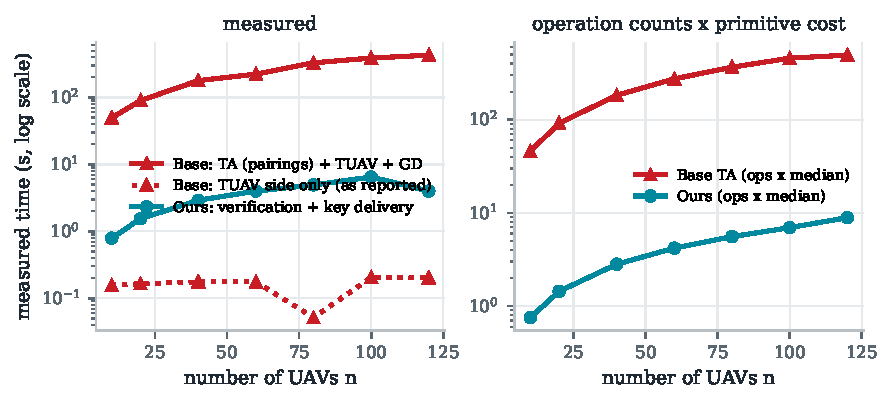
\includegraphics[width=\linewidth]{f2_latency}
\caption{E2: time to authenticate and key $n$ UAVs (log scale). Left: measured. Right: operation counts $\times$ median costs.}
\label{fig:e2}
\end{figure}

\textbf{Latency (E2).} For $n=\RNmax$ our TUAV authenticates and keys the swarm in \ROursTotalS\,s; the base scheme needs \RBaseTotalS\,s before any
satellite delay, and its TUAV-only part (the part~\cite{base} reports) is \RBaseTuavShare\% of that. By operation count the base scheme does
\RCountRatioLo--\RCountRatioHi$\times$ more work at every $n$; measured ratios ($n\le100$) are \RMeasRatioLo--\RMeasRatioHi$\times$. With the base paper's MIRACL constants the
figures are 228\,ms against 3720\,ms plus RTT (Fig.~\ref{fig:e2}).

\textbf{Availability (E1).} The base scheme succeeds in a fraction $A$ of rounds; with three retries at $A=50\%$ it reaches \RAvailIidHalfThree\% under independent
losses but only \RAvailBurstHalfThree\% under bursty outages. Ours does not use the link.

\begin{figure}[t]
\centering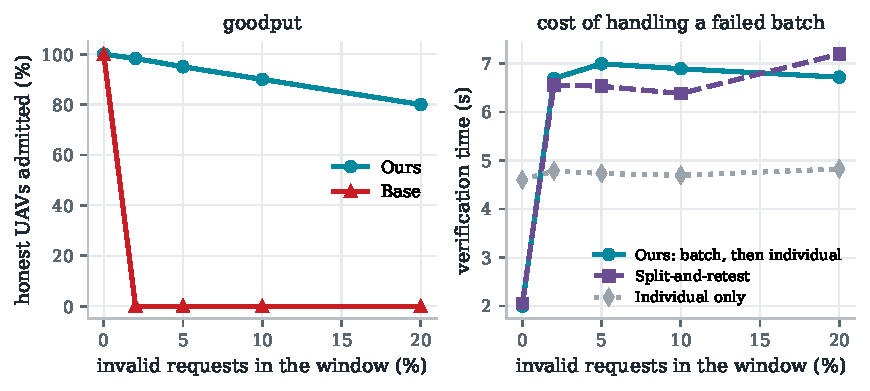
\includegraphics[width=\linewidth]{f3_poisoning}
\caption{E3: honest UAVs admitted and verification time under batch poisoning ($n=\RPoisonN$).}
\label{fig:e3}
\end{figure}

\textbf{Poisoning (E3).} One invalid request blocks every honest UAV in the base scheme. Ours admits all honest UAVs at every attack rate, with the cost bounded
by a failed batch plus individual checks (\RPoisonClean\,s clean, \RPoisonWorst\,s worst). Split-and-retest~\cite{zaverucha} brings no gain because pairing-free
batching is only a few times cheaper per signature (Fig.~\ref{fig:e3}).

\textbf{Traffic (E4).} For $n=120$ the base scheme's acknowledgements carry \RBytesBaseKey\,MB of CRT coefficients and it moves \RBytesBaseSat\,KB over the
satellite link. Our single ACK is \RBytesOursKey\,KB (\RBytesRatio$\times$ less). Our join request is larger (\RReqOurs\,B against \RReqBase\,B).

\textbf{Vehicles and handover (E5, E6).} A bundle of \RVehN\ vehicles is admitted, including keys, in \RVehBatchS\,s, and non-member bundles are dropped in
microseconds. A ticket handover costs the new TUAV \RHoTuavTicket\,ms instead of \RHoTuavFull\,ms. Over a one-hour mobility run with \RHoCross\ cell crossings,
the mean service gap falls from \RHoGapFull\,ms to \RHoGapTicket\,ms.

% =====================================================================
\section{Limitations}
A malicious TA keeps Girault level-2 power (detectable key replacement and phantom enrolment). A captured TUAV exposes its own cell's keys until it is
evicted. Pseudonyms are linkable within an epoch. Requests are larger. Our timings come from a pure-Python library on a laptop, and network effects are
simulated. Threshold TUAV trust, manufacturer-bound keys (level~3) and an embedded constant-time implementation are future work.

\section{Conclusion}
The TUAV architecture of~\cite{base} is a good answer to infrastructure loss, but its protocol keeps the cloud authority inside every step. Moving the trust
root offline restores infrastructure independence, escrow-freeness, forward secrecy and secure revocation together, reduces total work and traffic, and
extends naturally to vehicles and to multi-TUAV handover.

\begin{thebibliography}{10}
\bibitem{base} H.~Tan, W.~Zheng and P.~Vijayakumar, ``Secure and efficient authenticated key management scheme for UAV-assisted infrastructure-less IoVs,''
  \emph{IEEE Trans. Intell. Transp. Syst.}, vol.~24, no.~6, pp.~6389--6400, 2023.
\bibitem{alriyami} S.~S.~Al-Riyami and K.~G.~Paterson, ``Certificateless public key cryptography,'' in \emph{Proc. ASIACRYPT}, LNCS 2894, 2003, pp.~452--473.
\bibitem{girault} M.~Girault, ``Self-certified public keys,'' in \emph{Proc. EUROCRYPT}, LNCS 547, 1991, pp.~490--497.
\bibitem{bgr} M.~Bellare, J.~A.~Garay and T.~Rabin, ``Fast batch verification for modular exponentiation and digital signatures,'' in \emph{Proc. EUROCRYPT},
  LNCS 1403, 1998, pp.~236--250.
\bibitem{zaverucha} G.~M.~Zaverucha and D.~R.~Stinson, ``Group testing and batch verification,'' in \emph{Proc. ICITS}, LNCS 5973, 2009, pp.~140--157.
\bibitem{lkh} C.~K.~Wong, M.~Gouda and S.~S.~Lam, ``Secure group communications using key graphs,'' \emph{IEEE/ACM Trans. Netw.}, vol.~8, no.~1, pp.~16--30, 2000.
\bibitem{securelock} G.-H.~Chiou and W.-T.~Chen, ``Secure broadcasting using the secure lock,'' \emph{IEEE Trans. Softw. Eng.}, vol.~15, no.~8, pp.~929--934, 1989.
\bibitem{forking} D.~Pointcheval and J.~Stern, ``Security arguments for digital signatures and blind signatures,'' \emph{J. Cryptology}, vol.~13, no.~3,
  pp.~361--396, 2000.
\bibitem{proverif} B.~Blanchet, ``Modeling and verifying security protocols with the applied pi calculus and ProVerif,'' \emph{Found. Trends Priv. Secur.},
  vol.~1, no.~1--2, pp.~1--135, 2016.
\end{thebibliography}

\end{document}
